\documentclass[14pt]{extarticle}

\usepackage[T1]{fontenc}

\usepackage[main=greek,english]{babel}
\usepackage[utf8]{inputenc}
\usepackage[unicode]{hyperref}
\usepackage{titlepic}
\usepackage{graphicx}
\usepackage{listings}
\usepackage{xcolor}
\usepackage{amsmath}

\graphicspath{ {./img/} }

\usepackage{fontspec}
\setmainfont{CMU Serif}
\setsansfont{CMU Sans Serif}
\newfontfamily{\greekfont}{CMU Serif}
\newfontfamily{\greekfontsf}{CMU Sans Serif}
\usepackage{polyglossia}
\setdefaultlanguage{greek}

\hyphenpenalty=10000
\hbadness=10000

\definecolor{codegreen}{rgb}{0,0.6,0}
\definecolor{codegray}{rgb}{0.5,0.5,0.5}
\definecolor{codepurple}{rgb}{0.58,0,0.82}
\definecolor{backcolour}{rgb}{0.95,0.95,0.92}

\lstdefinestyle{mystyle}{
    backgroundcolor=\color{backcolour},   
    commentstyle=\color{codegreen},
    keywordstyle=\color{magenta},
    numberstyle=\tiny\color{codegray},
    stringstyle=\color{codepurple},
    basicstyle=\ttfamily\footnotesize,
    breakatwhitespace=false,         
    breaklines=true,                 
    captionpos=b,                    
    keepspaces=true,                 
    numbers=left,                    
    numbersep=5pt,                  
    showspaces=false,                
    showstringspaces=false,
    showtabs=false,                  
    tabsize=2
}

\lstset{frame=shadowbox, framexleftmargin=4mm, rulesepcolor=\color{black}, style=mystyle}

\title{\bf Σημειώσεις για αρχεία και φακέλους \\ Τμήμα B2}
\titlepic{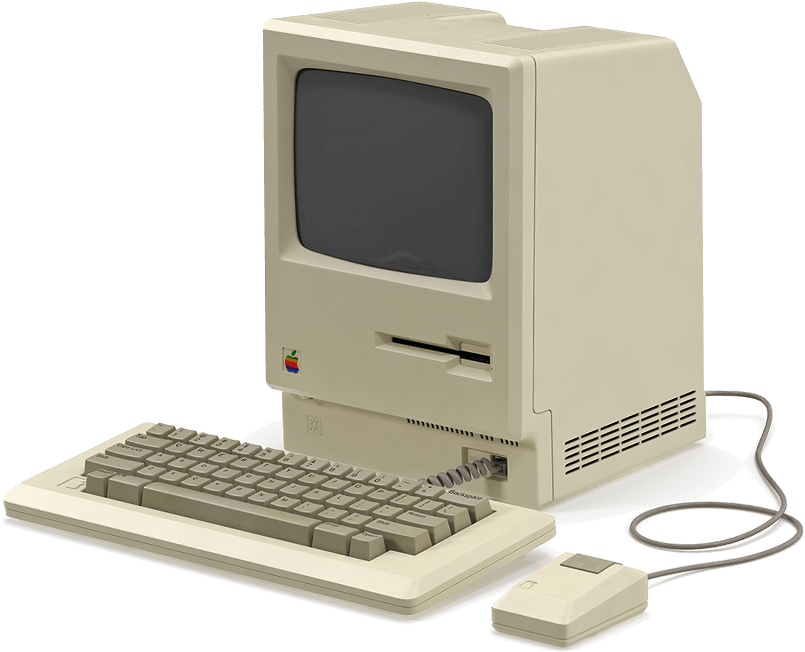
\includegraphics[scale=2.5]{computer.png}}
\author{
  \emph{Διονύσης Νικολόπουλος}
}

\begin{document}
\maketitle
Σημειώσεις για τους φακέλους που βρίσκονται στον κατάλογο υποβολής:
\begin{itemize}
\item \texttt{\textbf{bison-part}}:
Σε αυτόν τον κατάλογο βρίσκονται τα αρχεία πηγαίου κώδικα του bison.
\item \texttt{\textbf{flex-part}}:
Σε αυτόν τον κατάλογο βρίσκονται τα αρχεία πηγαίου κώδικα του flex.
\item \texttt{\textbf{compile-room}}:
Σε αυτόν τον κατάλογο βρίσκεται το makefile, το οποίο αντιγράφει τα απαραίτητα
αρχεία από τους προαναφερόμενους δύο καταλόγους στον τρέχοντα (compile-room),
και με αυτά τα αρχεία κάνει compile στο τελικό μας πρόγραμμα, που ονομάζεται
uni-c-analyser.
\end{itemize}
Επιπλέον, στον αρχικό κατάλογο υποβολής βρίσκεται και η εργασία, (υπεύθυνος για 
το τμήμα Β2: Αριστείδης Αναγνωστόπουλος), όπως και το αρχείο PDF αυτό που
διαβάζετε αυτή την στιγμή.
\end{document}

